% Options for packages loaded elsewhere
\PassOptionsToPackage{unicode}{hyperref}
\PassOptionsToPackage{hyphens}{url}
%
\documentclass[
]{article}
\usepackage{amsmath,amssymb}
\usepackage{iftex}
\ifPDFTeX
  \usepackage[T1]{fontenc}
  \usepackage[utf8]{inputenc}
  \usepackage{textcomp} % provide euro and other symbols
\else % if luatex or xetex
  \usepackage{unicode-math} % this also loads fontspec
  \defaultfontfeatures{Scale=MatchLowercase}
  \defaultfontfeatures[\rmfamily]{Ligatures=TeX,Scale=1}
\fi
\usepackage{lmodern}
\ifPDFTeX\else
  % xetex/luatex font selection
\fi
% Use upquote if available, for straight quotes in verbatim environments
\IfFileExists{upquote.sty}{\usepackage{upquote}}{}
\IfFileExists{microtype.sty}{% use microtype if available
  \usepackage[]{microtype}
  \UseMicrotypeSet[protrusion]{basicmath} % disable protrusion for tt fonts
}{}
\makeatletter
\@ifundefined{KOMAClassName}{% if non-KOMA class
  \IfFileExists{parskip.sty}{%
    \usepackage{parskip}
  }{% else
    \setlength{\parindent}{0pt}
    \setlength{\parskip}{6pt plus 2pt minus 1pt}}
}{% if KOMA class
  \KOMAoptions{parskip=half}}
\makeatother
\usepackage{xcolor}
\usepackage[margin=1in]{geometry}
\usepackage{color}
\usepackage{fancyvrb}
\newcommand{\VerbBar}{|}
\newcommand{\VERB}{\Verb[commandchars=\\\{\}]}
\DefineVerbatimEnvironment{Highlighting}{Verbatim}{commandchars=\\\{\}}
% Add ',fontsize=\small' for more characters per line
\usepackage{framed}
\definecolor{shadecolor}{RGB}{248,248,248}
\newenvironment{Shaded}{\begin{snugshade}}{\end{snugshade}}
\newcommand{\AlertTok}[1]{\textcolor[rgb]{0.94,0.16,0.16}{#1}}
\newcommand{\AnnotationTok}[1]{\textcolor[rgb]{0.56,0.35,0.01}{\textbf{\textit{#1}}}}
\newcommand{\AttributeTok}[1]{\textcolor[rgb]{0.13,0.29,0.53}{#1}}
\newcommand{\BaseNTok}[1]{\textcolor[rgb]{0.00,0.00,0.81}{#1}}
\newcommand{\BuiltInTok}[1]{#1}
\newcommand{\CharTok}[1]{\textcolor[rgb]{0.31,0.60,0.02}{#1}}
\newcommand{\CommentTok}[1]{\textcolor[rgb]{0.56,0.35,0.01}{\textit{#1}}}
\newcommand{\CommentVarTok}[1]{\textcolor[rgb]{0.56,0.35,0.01}{\textbf{\textit{#1}}}}
\newcommand{\ConstantTok}[1]{\textcolor[rgb]{0.56,0.35,0.01}{#1}}
\newcommand{\ControlFlowTok}[1]{\textcolor[rgb]{0.13,0.29,0.53}{\textbf{#1}}}
\newcommand{\DataTypeTok}[1]{\textcolor[rgb]{0.13,0.29,0.53}{#1}}
\newcommand{\DecValTok}[1]{\textcolor[rgb]{0.00,0.00,0.81}{#1}}
\newcommand{\DocumentationTok}[1]{\textcolor[rgb]{0.56,0.35,0.01}{\textbf{\textit{#1}}}}
\newcommand{\ErrorTok}[1]{\textcolor[rgb]{0.64,0.00,0.00}{\textbf{#1}}}
\newcommand{\ExtensionTok}[1]{#1}
\newcommand{\FloatTok}[1]{\textcolor[rgb]{0.00,0.00,0.81}{#1}}
\newcommand{\FunctionTok}[1]{\textcolor[rgb]{0.13,0.29,0.53}{\textbf{#1}}}
\newcommand{\ImportTok}[1]{#1}
\newcommand{\InformationTok}[1]{\textcolor[rgb]{0.56,0.35,0.01}{\textbf{\textit{#1}}}}
\newcommand{\KeywordTok}[1]{\textcolor[rgb]{0.13,0.29,0.53}{\textbf{#1}}}
\newcommand{\NormalTok}[1]{#1}
\newcommand{\OperatorTok}[1]{\textcolor[rgb]{0.81,0.36,0.00}{\textbf{#1}}}
\newcommand{\OtherTok}[1]{\textcolor[rgb]{0.56,0.35,0.01}{#1}}
\newcommand{\PreprocessorTok}[1]{\textcolor[rgb]{0.56,0.35,0.01}{\textit{#1}}}
\newcommand{\RegionMarkerTok}[1]{#1}
\newcommand{\SpecialCharTok}[1]{\textcolor[rgb]{0.81,0.36,0.00}{\textbf{#1}}}
\newcommand{\SpecialStringTok}[1]{\textcolor[rgb]{0.31,0.60,0.02}{#1}}
\newcommand{\StringTok}[1]{\textcolor[rgb]{0.31,0.60,0.02}{#1}}
\newcommand{\VariableTok}[1]{\textcolor[rgb]{0.00,0.00,0.00}{#1}}
\newcommand{\VerbatimStringTok}[1]{\textcolor[rgb]{0.31,0.60,0.02}{#1}}
\newcommand{\WarningTok}[1]{\textcolor[rgb]{0.56,0.35,0.01}{\textbf{\textit{#1}}}}
\usepackage{graphicx}
\makeatletter
\def\maxwidth{\ifdim\Gin@nat@width>\linewidth\linewidth\else\Gin@nat@width\fi}
\def\maxheight{\ifdim\Gin@nat@height>\textheight\textheight\else\Gin@nat@height\fi}
\makeatother
% Scale images if necessary, so that they will not overflow the page
% margins by default, and it is still possible to overwrite the defaults
% using explicit options in \includegraphics[width, height, ...]{}
\setkeys{Gin}{width=\maxwidth,height=\maxheight,keepaspectratio}
% Set default figure placement to htbp
\makeatletter
\def\fps@figure{htbp}
\makeatother
\setlength{\emergencystretch}{3em} % prevent overfull lines
\providecommand{\tightlist}{%
  \setlength{\itemsep}{0pt}\setlength{\parskip}{0pt}}
\setcounter{secnumdepth}{-\maxdimen} % remove section numbering
\usepackage{booktabs}
\usepackage{longtable}
\usepackage{array}
\usepackage{multirow}
\usepackage{wrapfig}
\usepackage{float}
\usepackage{colortbl}
\usepackage{pdflscape}
\usepackage{tabu}
\usepackage{threeparttable}
\usepackage{threeparttablex}
\usepackage[normalem]{ulem}
\usepackage{makecell}
\usepackage{xcolor}
\usepackage{caption}
\ifLuaTeX
  \usepackage{selnolig}  % disable illegal ligatures
\fi
\IfFileExists{bookmark.sty}{\usepackage{bookmark}}{\usepackage{hyperref}}
\IfFileExists{xurl.sty}{\usepackage{xurl}}{} % add URL line breaks if available
\urlstyle{same}
\hypersetup{
  pdftitle={Text Analysis},
  pdfauthor={Saurab den Butter},
  hidelinks,
  pdfcreator={LaTeX via pandoc}}

\title{Text Analysis}
\usepackage{etoolbox}
\makeatletter
\providecommand{\subtitle}[1]{% add subtitle to \maketitle
  \apptocmd{\@title}{\par {\large #1 \par}}{}{}
}
\makeatother
\subtitle{Weekly assignment 6}
\author{Saurab den Butter}
\date{02 November, 2023}

\begin{document}
\maketitle

{
\setcounter{tocdepth}{1}
\tableofcontents
}
\hypertarget{loading-required-packages-for-the-analysis}{%
\section{\texorpdfstring{\textbf{Loading required packages for the
analysis}}{Loading required packages for the analysis}}\label{loading-required-packages-for-the-analysis}}

I start by loading the required packages for the analysis.

\begin{Shaded}
\begin{Highlighting}[]
\DocumentationTok{\#\# Load required packages {-}{-}{-}{-}}
\ControlFlowTok{if}\NormalTok{(}\SpecialCharTok{!}\FunctionTok{require}\NormalTok{(pacman))\{}
        \FunctionTok{install.packages}\NormalTok{(}\StringTok{\textquotesingle{}pacman\textquotesingle{}}\NormalTok{)}
\NormalTok{\}}

\FunctionTok{p\_load}\NormalTok{(tidyverse, tm, textclean, }
\NormalTok{       gt, janitor, ggthemes,}
\NormalTok{       kableExtra, SnowballC,}
\NormalTok{       RColorBrewer, wordcloud)}

\FunctionTok{theme\_set}\NormalTok{(ggthemes}\SpecialCharTok{::}\FunctionTok{theme\_clean}\NormalTok{())}
\FunctionTok{options}\NormalTok{(}\AttributeTok{digits =} \DecValTok{3}\NormalTok{)}
\FunctionTok{options}\NormalTok{(}\AttributeTok{scipen =} \DecValTok{999}\NormalTok{)}
\end{Highlighting}
\end{Shaded}

\hypertarget{question-3-stack-exchange-topics-and-questions}{%
\section{\texorpdfstring{\textbf{Question 3: Stack Exchange topics and
questions}}{Question 3: Stack Exchange topics and questions}}\label{question-3-stack-exchange-topics-and-questions}}

Over the years, Facebook has hosted multiple competitions on
\texttt{Kagle} to recruit new employees. This question is based on the
third challenge.2 . The original competition tested text mining skills
on a large data set from the Stack Exchange sites. The task was to
predict the tags (a.k.a. keywords, topics, summaries), given only the
question text and its title. The data set contains content from
disparate stack exchange sites, containing a mix of both technical and
non-technical questions. A sample of this data set has been made
available on Canvas, as stack.csv, and this sample provides three
columns: the Topic of the post (one of four topics), the Title of the
post, and the Body of the post which contains the actual question and
explanation. This data set will be used for the rest of the assignment.

\hypertarget{distribution-of-posts-over-the-various-topics}{%
\subsection{Distribution of posts over the various
topics}\label{distribution-of-posts-over-the-various-topics}}

The data set has 2626 observations and 3 variables.

\begin{longtable}{lrr}
\toprule
TOPIC & COUNT & Prop \\ 
\midrule\addlinespace[2.5pt]
Facebook & 982 & 0.374 \\ 
Security & 661 & 0.252 \\ 
Excel & 617 & 0.235 \\ 
Firefox & 366 & 0.139 \\ 
\bottomrule
\end{longtable}

The topic about \texttt{Facebook} is the most prevalent with 982 entries
that accounts for about 37\% of the observations. \texttt{Security}
matters are also prominent with 661 observations (about 25\%) of the
posts. Posts about \texttt{Excel} and \texttt{Firefox} are the least
prevalent with 617 (24\%) and 366 (14\%) prevalence, respectively.

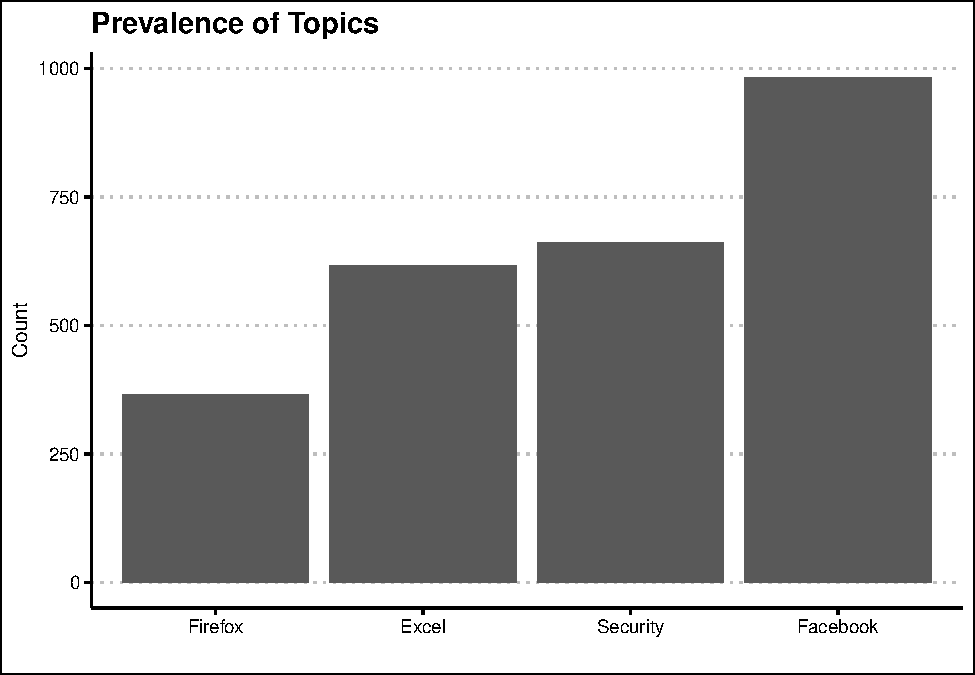
\includegraphics{assign6_files/figure-latex/unnamed-chunk-5-1.pdf}

\hypertarget{inspect-a-couple-of-question-text-bodies-and-report-on-your-observations}{%
\subsection{Inspect a couple of question text bodies and report on your
observations}\label{inspect-a-couple-of-question-text-bodies-and-report-on-your-observations}}

The topic section contains HTML tags like \textless p\textgreater{} and
\textless\textbackslash p\textgreater{} and URLs for various websites
referred to in the text. The text also contains digits that may not be
of much use in a text analysis. Moreover, the existence of punctuation
and, as in standard grammar, we have a mix of upper case and lower case
letters in spelling of words (like at the start of a sentence). This
could make two otherwise similar word be different. We also have a lot
of special characters (like *, \#, @, \%) that carry no meaning in text
analysis. White spaces, and line breaks are also prevalent. Importantly,
we have words that are indispensable in language but that carry no
meaning on their own (called stop-words, for example the articles
\texttt{a} and \texttt{the}, among others). p

\begin{verbatim}
## [1] "<p>In my favorite editor (vim), I regularly use ctrl-w to execute a certain action. Now, it quite often happens to me that firefox is the active window (on windows) while I still look at vim (thinking vim is the active window) and press ctrl-w which closes firefox. This is not what I want. Is there a way to stop ctrl-w from closing firefox?</p>\n\n<p>Rene</p>\n"                                                                                                                                                                                                                                                                                                                                                                                                                                                                                                                                                                                                                                                                                                                                                                                                                                                                                                                                                                                                                                                                                                                                                                                                                                                                                             
## [2] "<p>Aloha everyone,</p>\n\n<p>I have a class assignment in which I am tasked to build a MySql database, then use PHP to retrieve the contents of the table in the database.  When I attempt to open this in Safari, it only outputs the HTML/PHP code.  Firefox, on the other hand, pops up a window asking me to select an application to work with the code.  Here is the code itself.  Can anyone see where my error lies and/or point me in the right direction to get this actually interpreted and display correctly?  Any and all assistance will be greatly appreciated.</p>\n\n<pre><code>&lt;html&gt;\n &lt;head&gt;\n  &lt;title&gt;iBud's Sizzling Tracks!&lt;/title&gt;\n &lt;/head&gt;\n &lt;body&gt;\n &lt;?php\n  $con = mysql_connct(\"localhost\",\"*****\",\"**************\");\n  if (!$con) {\n    die('Could not connect: ' . mysql_error());\n    }\n\n  mysql_select_db(\"music\", $con);\n\n  $result = mysql_query(\"SELECT * FROM songs\");\n\n  echo \"&lt;table border='1'&gt;\n  &lt;tr&gt;\n  &lt;th&gt;Song Number&lt;/th&gt;\n  &lt;th&gt;Song Title&lt;/th&gt;\n  &lt;th&gt;Artist&lt;/th&gt;\n  &lt;th&gt;Rating&lt;/th&gt;\n  &lt;/tr&gt;\";\n\n  while ($row = mysql_fetch_array($result)) {\n    echo \"&lt;tr&gt;\";\n    echo \"&lt;td&gt;\" . $row['songNumber'] . \"&lt;/td&gt;\";\n    echo \"&lt;td&gt;\" . $row['songTitle'] . \"&lt;/td&gt;\";\n    echo \"&lt;td&gt;\" . $row['artistName'] . \"&lt;/td&gt;\";\n    echo \"&lt;td&gt;\" . $row['rating'] . \"&lt;/td&gt;\";\n    echo \"&lt;/tr&gt;\";\n    }\n  echo \"&lt;/table&gt;\";\n\n  mysql_close($con);\n  ?&gt;\n &lt;/body&gt;\n&lt;/html&gt;\n</code></pre>\n"
## [3] "<p>I recently started using Firefox as my primary web browser, and I would like to change some of the default keyboard shortcuts, especially the ones used to switch between tabs. Can this be done?</p>\n\n<p>I took a peek through the Firefox directory in \"Application Support\", as well as the application bundle itself, but nothing jumped out. Google searches have also proved fruitless.</p>\n\n<p>Any help is appreciated!</p>\n\n<p><em><strong>Update:</em></strong> I'm running Firefox version 3.6 for Mac OS 10.6.2</p>\n"                                                                                                                                                                                                                                                                                                                                                                                                                                                                                                                                                                                                                                                                                                                                                                                                                                                                                                                                                                                                                                                                                                                             
## [4] "<p>I stepped over the following tutorial:\n<a href=\"http://afana.me/post/create-wizard-in-aspnet-mvc-3.aspx\" rel=\"nofollow\">http://afana.me/post/create-wizard-in-aspnet-mvc-3.aspx</a></p>\n\n<p>Since it looks pretty nice, I'm asking myself if making the complete wizard in JavaScript just like that is a good/safe idea?</p>\n"                                                                                                                                                                                                                                                                                                                                                                                                                                                                                                                                                                                                                                                                                                                                                                                                                                                                                                                                                                                                                                                                                                                                                                                                                                                                                                                               
## [5] "<p>The site is set to WordPress 3.4.1, annexed widget Facebook for WordPress</p>\n\n<p>Later I changed the name to the Facebook user profile, and now get an error that I need to reference a valid Facebook user profile.</p>\n\n<p>What changes do I have to make so that data-href will be the correct (new) Facebook user profile? Can you guide me? </p>\n"
\end{verbatim}

\hypertarget{discuss-issues-that-need-to-be-solved-when-cleaning-the-text-later-on.}{%
\subsubsection{Discuss issues that need to be solved when cleaning the
text later
on.}\label{discuss-issues-that-need-to-be-solved-when-cleaning-the-text-later-on.}}

\begin{enumerate}
\def\labelenumi{\arabic{enumi}.}
\item
  HTML Tags: Because the text data comes from web sources, it contains
  HTML tags. I will remove these tags before commencing analysis.
\item
  Convert text to lower case: I will convert all text to lowercase to
  ensure consistency and prevent case-sensitive issues.
\item
  Punctuation: I will remove all punctuation marks (e.g., periods,
  commas, quotes) as they may not provide valuable information for
  analysis.
\item
  Special Characters: I will eliminate special characters, such as
  currency symbols or trademark signs, which may not be relevant to our
  analysis.
\item
  Stop Words: I will remove common stopwords (e.g., ``and,'' ``the,''
  ``in'') as they often don't carry significant meaning for analysis.
  The \texttt{tm} package contains the list of the common English
  stopwords.
\item
  Numeric Character Removal: Because numbers are not relevant to our
  analysis, we remove them from the text. This is useful because we are
  focusing on language and not numerical data.
\item
  Whitespace and Line Breaks: I will remove extra whites pace and line
  breaks to ensure uniform formatting of the text before analysis.
  Without this, white spaces and line breaks could be mistaken for words
  and hence cloud our analysis.
\item
  Remove URLs: The text contains web links. I remove these links as they
  are not relevant to our analysis.
\item
  Tokenization: I will tokenize the text into words or phrases (tokens)
  to prepare it for further analysis.
\item
  Contractions: Some contractions in language complicate the analysis.
  In that case, I will replace all contractions into standard language
  (for instance, I'll to I will).
\item
  Finally, I will be on the lookout for irrelevant meta data and
  non-standard character encoding that could affect the analysis.
\end{enumerate}

\hypertarget{question-4-preparation-of-the-text}{%
\section{\texorpdfstring{\textbf{Question 4: Preparation of the
text}}{Question 4: Preparation of the text}}\label{question-4-preparation-of-the-text}}

Choose two of the Topics for use in the rest of the assignment. Prepare
(cleanse) the question body texts for further analysis by means of the
following steps.

I select the following TWO topics;

\begin{itemize}
\item
  Facebook.
\item
  Security.
\end{itemize}

\hypertarget{use-functions-from-package-textclean-to-remove-urls-and-make-other-desired-adjustments.}{%
\subsection{Use functions from package textclean to remove URLs and make
other desired
adjustments.}\label{use-functions-from-package-textclean-to-remove-urls-and-make-other-desired-adjustments.}}

To clean the data, I create a function that will automatically deal with
all the issues identified above.

I use the above function to clean the data. I start with the facebook
topic data.

Next, I clean the security topic data.

\hypertarget{use-package-tm-to-build-a-corpus-from-the-vector-with-cleansed-text-for-each-of-your-chosen-topic}{%
\subsection{Use package tm to build a corpus from the vector with
cleansed text for each of your chosen
Topic;}\label{use-package-tm-to-build-a-corpus-from-the-vector-with-cleansed-text-for-each-of-your-chosen-topic}}

In this section, I build a corpus and implement several cleansing steps
as follow;

\begin{enumerate}
\def\labelenumi{\arabic{enumi}.}
\item
  I remove all the English stopwords as described earlier. These words
  are important in grammar but carry no meaning on their own.
\item
  I remove all the numbers as they are not relevant in our text
  analysis.
\item
  Further, I eliminate all punctuation. Punctuation does not add value
  to a text analysis.
\item
  Next, I convert all text to lower case so that case sensitivity does
  not negatively affect our analysis.
\item
  Finally, I strip all the extra white spaces between words.
\end{enumerate}

I then convert the output into a term document matrix.

\hypertarget{number-of-words-and-documents-in-the-resulting-corpus-for-each-of-your-chosen-topic.}{%
\subsection{Number of words and documents in the resulting corpus for
each of your chosen
Topic.}\label{number-of-words-and-documents-in-the-resulting-corpus-for-each-of-your-chosen-topic.}}

The facebook topic consists of one document with 9517 terms. There is
zero sparse terms, meaning that each of the terms appears at least once.
The maximal term length is 368.

\begin{verbatim}
## <<TermDocumentMatrix (terms: 9517, documents: 1)>>
## Non-/sparse entries: 9517/0
## Sparsity           : 0%
## Maximal term length: 368
## Weighting          : term frequency (tf)
\end{verbatim}

The facebook topic consists of one document with 8647 terms. There is
zero sparse terms, meaning that each of the terms appears at least once.
The maximal term length is 676.

\begin{verbatim}
## <<TermDocumentMatrix (terms: 8647, documents: 1)>>
## Non-/sparse entries: 8647/0
## Sparsity           : 0%
## Maximal term length: 676
## Weighting          : term frequency (tf)
\end{verbatim}

\hypertarget{question-5-popular-associates}{%
\section{\texorpdfstring{\textbf{Question 5: Popular
associates}}{Question 5: Popular associates}}\label{question-5-popular-associates}}

For each of your chosen Topic, make an overview of the most frequent
terms in the corpus and make an overview of the terms that have the
higher correlations with that Topic. Comment on the results. Speculate
as to whether there is possible predictive value in these results.
{[}0.5 page{]}

In each case, I pick the terms that occur at least 400 times, starting
with the Facebook topic below.

\begin{verbatim}
##  [1] "app"      "can"      "code"     "facebook" "frown"    "get"     
##  [7] "like"     "page"     "pnn"      "post"     "skeptic"  "stick"   
## [13] "tongu"    "tri"      "use"      "user"     "work"
\end{verbatim}

Next, we look at the security topic.

\begin{verbatim}
## [1] "can"     "frown"   "secur"   "server"  "skeptic" "stick"   "tongu"  
## [8] "use"     "user"
\end{verbatim}

We see a clear distinction in the terms occurring in both topics. For
the security topic, the terms \texttt{secur} has a high association with
the topic. For Facebook, the term \texttt{facebook}, \texttt{app} have a
high correlation with the topic. In our case, the terms ``can'',
``skeptic'', ``use'', and ``User'' have little predictive value in topic
modelling. Overall, the output has some predictive power as there are
words that clearly stand out in each of the topics. For instance, the
term \texttt{server} is highly related to the security topic but is not
among the top terms in the facebook topic. Likewise, the term
\texttt{page} is more prevalent in the facebook topic than in the
security topic. Such prevalence of terms gives rise the data some
predictive power.

\hypertarget{question-6-word-clouds}{%
\section{\texorpdfstring{\textbf{Question 6: Word
clouds}}{Question 6: Word clouds}}\label{question-6-word-clouds}}

Make a word cloud for each of your chosen Topic, and include these in
your report. Compare the two graphs and discuss the result. {[}0.5
page{]}

I make a word cloud for each of the topics. Figure 2 shows the word
cloud for the facebook topic while Figure 3 shows one for the security
topic. In each case, we see that although there are commonalities in the
word clouds, some terms clearly stand out in each of the topics. For
instance, the term \texttt{Facebook} stand out in the facebook topic.
The terms \texttt{secur} and \texttt{app} appears more in the security
topic. There are some overlaps though. The terms \texttt{skeptic},
\texttt{user} and \texttt{use} are common in both topics. However, this
overlap does not take away the usefulness of the data for predictive
modelling.

Other terms that stand out in the facebook topic.

\begin{itemize}
\tightlist
\item
  Like.
\item
  Page.
\item
  frown.
\end{itemize}

Other terms that stand out in the security topic.

\begin{itemize}
\tightlist
\item
  Server.
\item
  Password.
\item
  Access.
\item
  Data.
\end{itemize}

Terms that overlap in both topics include, among others the following:

\begin{itemize}
\tightlist
\item
  Use.
\item
  User.
\item
  Code.
\item
  Skeptic.
\end{itemize}

\hypertarget{world-cloud-for-facebook-topic}{%
\subsubsection{World Cloud for Facebook
Topic}\label{world-cloud-for-facebook-topic}}

\begin{figure}
\centering
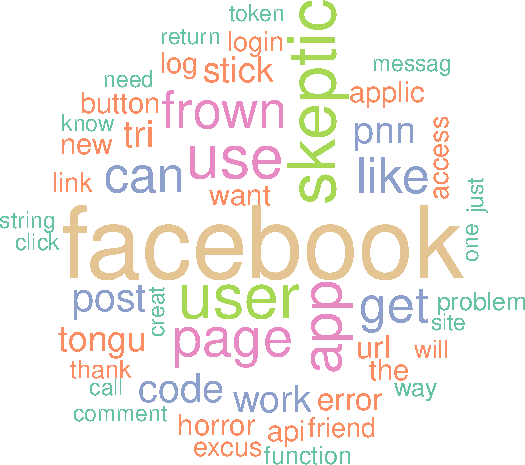
\includegraphics{assign6_files/figure-latex/unnamed-chunk-17-1.pdf}
\caption{WordCloud for the Facebook Topic}
\end{figure}

\newpage

\hypertarget{world-cloud-for-security-topic}{%
\subsubsection{World Cloud for Security
Topic}\label{world-cloud-for-security-topic}}

\begin{figure}
\centering
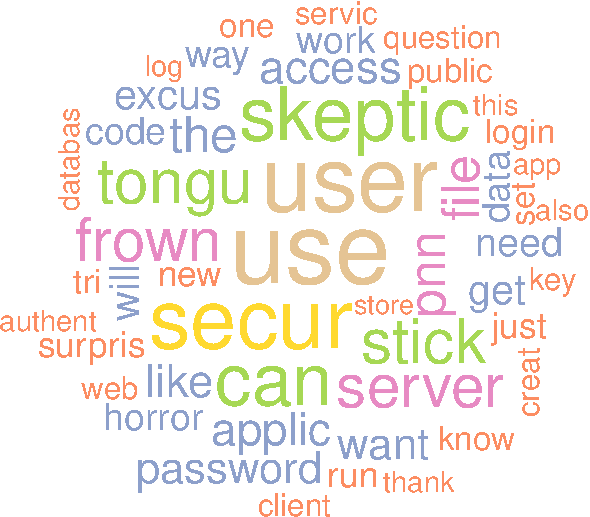
\includegraphics{assign6_files/figure-latex/unnamed-chunk-19-1.pdf}
\caption{WordCloud for the Security Topic}
\end{figure}

\newpage

\hypertarget{references}{%
\section{\texorpdfstring{\textbf{References}}{References}}\label{references}}

Banks, G. C., Woznyj, H. M., Wesslen, R. S., \& Ross, R. L. (2018). A
review of best practice recommendations for text analysis in R (and a
user-friendly app). \textbf{Journal of Business and Psychology}, 33,
445-459.

Welbers, K., Van Atteveldt, W., \& Benoit, K. (2017). Text analysis in
R. \textbf{Communication methods and measures}, 11(4), 245-265.

\hypertarget{code-appendix}{%
\section{\texorpdfstring{\textbf{Code
Appendix}}{Code Appendix}}\label{code-appendix}}

\begin{verbatim}
## ----setup, include=FALSE----------------------------------------------------------------------------
knitr::opts_chunk$set(echo = FALSE, warning = FALSE, message = FALSE)



## ----echo = TRUE-------------------------------------------------------------------------------------
## Load required packages ----
if(!require(pacman)){
        install.packages('pacman')
}

p_load(tidyverse, tm, textclean, 
       gt, janitor, ggthemes,
       kableExtra, SnowballC,
       RColorBrewer, wordcloud)

theme_set(ggthemes::theme_clean())
options(digits = 3)
options(scipen = 999)


## ----------------------------------------------------------------------------------------------------
## Load the data ----
chats <- read_csv('stack.csv') %>% 
        clean_names()


## ----------------------------------------------------------------------------------------------------
## Topics ----
counts <- chats %>% 
        count(topic, 
              sort = TRUE, 
              name = "Count")



## ----------------------------------------------------------------------------------------------------
## Prevalent topics table ----
counts %>% 
        set_names(names(.) %>% str_to_upper()) %>% 
        mutate(Prop = COUNT / nrow(chats)) %>% 
        gt(caption = "Prevalence of Topics")
        


## ----------------------------------------------------------------------------------------------------
## Prevalent topics ----
counts %>% 
        mutate(topic = fct_reorder(topic, Count)) %>% 
        ggplot(mapping = aes(x = topic, y = Count)) + 
        geom_col() + 
        labs(x = "", title = "Prevalence of Topics")


## ----------------------------------------------------------------------------------------------------
## Chats body overview ----
chats %>% 
        pull(body) %>% 
        head(5)


## ----------------------------------------------------------------------------------------------------
## text cleaning function using text clean ----
text_cleaner <- function(text){
        library(textclean)
        library(tidyverse)
        text %>% 
                replace_contraction() %>% 
                replace_date(replacement = "") %>% 
                replace_email() %>% 
                replace_emoji() %>% 
                replace_emoticon() %>% 
                replace_hash() %>% 
                replace_html() %>% 
                replace_internet_slang() %>% 
                replace_white() %>% 
                replace_number(remove = TRUE) %>% 
                replace_tag() %>% 
                replace_url() %>% 
                replace_word_elongation()
}


## ----------------------------------------------------------------------------------------------------
## Clean facebook data ----
clean_fb <- chats %>% 
        filter(topic == "Facebook") %>% 
        select(body) %>% 
        text_cleaner()


## ----------------------------------------------------------------------------------------------------
## Clean security data ----
clean_sec <- chats %>% 
        filter(topic == "Security") %>% 
        select(body) %>% 
        text_cleaner()


## ----------------------------------------------------------------------------------------------------
## Create a document term matrix for facebook topic ----
fb_dtm <- clean_fb %>% 
        VectorSource() %>% 
        Corpus() %>% 
        tm_map(removeWords, stopwords('english')) %>% 
        tm_map(removeNumbers) %>% 
        tm_map(removePunctuation) %>% 
        tm_map(tolower) %>% 
        tm_map(stripWhitespace) %>% 
        tm_map(stemDocument) %>% 
        TermDocumentMatrix()
        


## ----------------------------------------------------------------------------------------------------
## Create a document term matrix for security topic ----
sec_dtm <- clean_sec %>% 
        VectorSource() %>% 
        Corpus() %>% 
        tm_map(removeWords, stopwords('english')) %>% 
        tm_map(removeNumbers) %>% 
        tm_map(removePunctuation) %>% 
        tm_map(tolower) %>% 
        tm_map(stripWhitespace) %>% 
        tm_map(stemDocument) %>% 
        TermDocumentMatrix()


## ----------------------------------------------------------------------------------------------------
## Documents and term counts in facebook topic ----
fb_dtm


## ----------------------------------------------------------------------------------------------------
## Documents and term counts in security topic ----
sec_dtm


## ----------------------------------------------------------------------------------------------------
## Popular terms- facebook ----
fb_dtm %>% 
        findFreqTerms(lowfreq = 400) %>% 
        head(30)


## ----------------------------------------------------------------------------------------------------
## Popular terms- security ----
sec_dtm %>% 
        findFreqTerms(lowfreq = 400) %>% 
        head(30)


## ----fig.cap="WordCloud for the Facebook Topic"------------------------------------------------------
## Wordcloud- facebook ----
fb_df <- fb_dtm %>% 
        as.matrix() %>% 
        data.frame() %>% 
        set_names("Count") %>% 
        mutate(Term = row.names(.)) %>% 
        arrange(desc(Count))

## Word cloud for facebook topic ----
wordcloud(
        words = fb_df$Term,
        freq = fb_df$Count,
         min.freq=1, 
         max.words = 50, 
         random.order = FALSE, 
         colors=brewer.pal(7, "Set2")) 


## ----fig.cap="WordCloud for the Security Topic"------------------------------------------------------
## Wordcloud- security ----
sec_df <- sec_dtm %>% 
        as.matrix() %>% 
        data.frame() %>% 
        set_names("Count") %>% 
        mutate(Term = row.names(.)) %>% 
        arrange(desc(Count))

## Word cloud for security topic ----
wordcloud(
        words = sec_df$Term,
        freq = sec_df$Count,
         min.freq=1, 
         max.words = 50, 
         random.order = FALSE, 
         colors=brewer.pal(7, "Set2")) 




\end{verbatim}

\end{document}
